\chapter{Analýza}

Cílem nového skladového systému je nahradit a rozšířit funkce stávajícího skladového systému Sysel - proto jsme při analýze požadavků vycházeli\footnote{Já a kolega Pavel Kovář, který se zabývá backendem nového systému} jednak z tohoto řešení a dále z požadavků primárního potenciálního zákazníka - jednoho ze současných uživatelů tohoto systému.\\
Současná verze Sysla je již oproti svému původnímu návrhu velmi upravena, a to se podepisuje na snížené možnosti dalších úprav a celkové komplexnosti systému.\\
Pro nový systém je na jedné straně důležité, aby bylo stále možné provádět ty procesy, které jsou ideální již za současného stavu. Na straně druhé je pak důležité zohlednit nové požadavky a pokusit se umožnit i snadné reakce na budoucí požadavky.

%%%%%%%%%%%%%%%%%%%%%%%%%%%%%%%%%%%%%%%%%%%%%%%%%%%%%%%%%%%%%%%%%%%%%%%%%%%%%%%%
%%%%%%%%%%%%%%%%%%%%%%%%%%%%%%%%%%%%%%%%%%%%%%%%%%%%%%%%%%%%%%%%%%%%%%%%%%%%%%%%
%%%%%%%%%%%%%%%%%%%%%%%%%%%%%%%%%%%%%%%%%%%%%%%%%%%%%%%%%%%%%%%%%%%%%%%%%%%%%%%%
%%%%%%%%%%%%%%%%%%%%%%%%%%%%%%%%%%%%%%%%%%%%%%%%%%%%%%%%%%%%%%%%%%%%%%%%%%%%%%%%

\section{Analýza požadavků dle současného systému}\label{sec:analysis}

Jádrem současného skladového systému je rozdělení na dvě role: skladník a vedoucí. Aplikace podporuje práci ve středně velkém skladu, který používá čárové kódy na zboží a umístěních, ale nemá další pokročilé automatizace jako například pohyb objednávkových bedýnek po páse, roboty, kteří autonomně vyzvedávají zboží atp. Veškeré pohyby jsou realizovány lidskými zdroji a tomu odpovídá i realizace podpůrného systému. Výhodou tohoto řešení je možnost použití systému i v menších skladech a to případně i o velikosti pouze jednoho správce.\\

\subsection{Funkční požadavky}

Role skladníka:
\begin{itemize}
	\item přijímat nové dodávky zboží,
	\item naskladňovat zboží,
	\item přesouvat zboží v rámci skladu,
	\item přesouvat celá umístění,
	\item vyskladňovat zboží,
	\item provést inventuru,
	\item zobrazovat úlohy.
\end{itemize}

Role vedoucího:
\begin{itemize}
	\item spravovat sklady,
	\item spravovat umístění ve skladech,
	\item spravovat výrobce,
	\item spravovat zboží,
	\item zadávat úlohy skladníkům,
	\item sledovat stav probíhajících a uzavřených úloh.
\end{itemize}

Tyto požadavky vychází ze stávající aplikace Sysel a jejich procesy měly zůstat zachovány, proto jsme konkrétní use-case a detailní procesy navrhli na základě průchodů současného systému. Diagramy, které jsou výstupem této části analýzy jsou součástí přílohy \ref{ap:diagram:storekeeper}.

%%%%%%%%%%%%%%%%%%%%%%%%%%%%%%%%%%%%%%%%%%%%%%%%%%%%%%%%%%%%%%%%%%%%%%%%%%%%%%%%
%%%%%%%%%%%%%%%%%%%%%%%%%%%%%%%%%%%%%%%%%%%%%%%%%%%%%%%%%%%%%%%%%%%%%%%%%%%%%%%%
%%%%%%%%%%%%%%%%%%%%%%%%%%%%%%%%%%%%%%%%%%%%%%%%%%%%%%%%%%%%%%%%%%%%%%%%%%%%%%%%
%%%%%%%%%%%%%%%%%%%%%%%%%%%%%%%%%%%%%%%%%%%%%%%%%%%%%%%%%%%%%%%%%%%%%%%%%%%%%%%%

\section{Analýza nových požadavků}

\subsection{Logistika}

Hlavním novým požadavkem, který současný Sysel nepodporuje, je správa \emph{logistiky} - tedy místa ve skladu, kde dochází ke kompletaci odchozího zboží, jeho balení atp.\\
Toto místo se od běžného skladového umístění odlišuje v tom, co se zde eviduje navíc:
\begin{itemize}
	\item \emph{Použitý spotřební materiál:} Zaznamenávají se spotřebované balíky či fólie, ale například i palety.
	\item \emph{Doba uložení:} Ukládá se, jak dlouho zde dané zboží \uv{zabíralo} místo.
	\item \emph{Činnosti skladníka:} Zde se eviduje, kolik a jaké úkony musel skladník se zbožím provést - jako například \emph{balení do folie}, \emph{přeskládání} atp.
\end{itemize}

\subsection{Evidence stráveného času}

Podobně jako se u Logistiky má ukládat čas, po který zboží leželo v Logistice, mělo by být možné v aplikaci celkově evidovat, kolik času strávil skladník jakým úkolem. Při přijetí úkolu se automaticky spustí stopky měřící strávený čas daným úkolem, také je ale nutné mít možnost stopky pozastavit - například během pauzy na oběd apod.\\
Časové přehledy skladníků by měly být použitelné jednak pro kontrolu výkonu skladníků, ale také pro potenciální fakturaci nákladů třetím stranám - pro případ, že by sklad provozoval jiný subjekt, než je reálný majitel zboží, který platí za uskladnění.

\subsection{Rozhraní pro nemobilní zařízení}

Současný systém je navržen mobile-first, což by mělo být zachováno - skladníci používají mobilní zařízení se zabudovanou čtečkou. Toto rozhraní se ale prakticky vůbec nezmění i při použití větší obrazovky - na tabletech je rozhraní ještě poměrně použitelné, ale na notebooku či stolním počítači je zobrazení přinejmenším \emph{neoptimalizované} - neexistuje zde žádná práce s horizontálním místem, vše je řazeno vertikálně. Jako ukázku přikládám screenshot úryvku domovské obrazovky vedoucího skladu (obrázek \ref{picture:sysel:vertical}), obsahující náhled na reálný stav používaného skladu, s anonymizovanými daty.\\
Požadavkem tedy je, aby rozhraní bylo plně responzivní - role skladníka sice typicky na počítači opravdu používána nebude, ale vedoucí skladu by měl mít možnost volně přecházet mezi různými zařízeními.

\begin{figure}[]
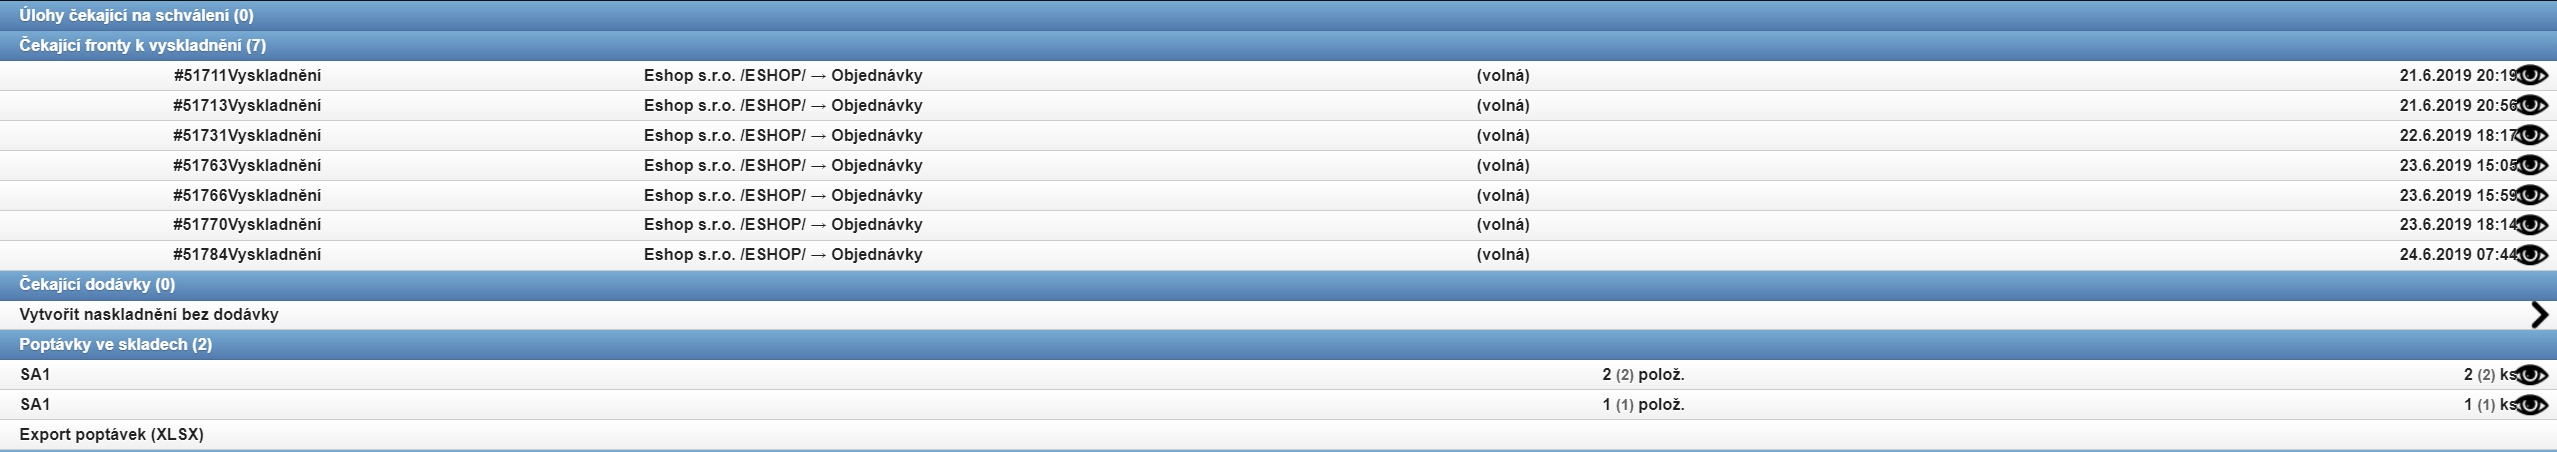
\includegraphics[width=\textwidth]{../png/sysel/vertical.png}
\caption{Ukázka špatné práce s horizontálním místem ve starém skladovém systému} \label{picture:sysel:vertical}
\end{figure}

%%%%%%%%%%%%%%%%%%%%%%%%%%%%%%%%%%%%%%%%%%%%%%%%%%%%%%%%%%%%%%%%%%%%%%%%%%%%%%%%
%%%%%%%%%%%%%%%%%%%%%%%%%%%%%%%%%%%%%%%%%%%%%%%%%%%%%%%%%%%%%%%%%%%%%%%%%%%%%%%%
%%%%%%%%%%%%%%%%%%%%%%%%%%%%%%%%%%%%%%%%%%%%%%%%%%%%%%%%%%%%%%%%%%%%%%%%%%%%%%%%
%%%%%%%%%%%%%%%%%%%%%%%%%%%%%%%%%%%%%%%%%%%%%%%%%%%%%%%%%%%%%%%%%%%%%%%%%%%%%%%%

\section{Analýza konkurence}

Před započetím tvorby nových návrhů UI je vhodné analyzovat existující konkurenční řešení.\\
V dnešní době existuje na trhu nespočet skladových systémů, jednak veřejně dostupných, které nabízejí buď zkušební verzi zdarma, nebo jsou placené, ale zato mají dostupný popis jejich vlastností, a pak také spousta uzavřených systémů, které si nechal někdo vytvořit na míru přesně pro své potřeby, a pro veřejnost není daný systém vůbec dostupný.\\
Z tohoto důvodu jsem se rozhodl zaměřit především na funkcinality veřejně dostupných skladových systémů, které jsou primárně určené na mobilní zařízení.\\

\subsection{Analýza mobilních aplikací pro evidenci skladu}

\subsubsection{Storage Manager: Stock Tracker}

Tuto aplikaci lze nalézt v Google Play Store a je k dispozici její varianta zdarma, kterou jsem také vyzkoušel.\\
Stejně jako Sysel umožňuje skenovat čárové kódy nejen na zboží, ale i na umístění. Má podobné možnosti manipulace se zbožím: naskladnění, vyskladnění, přesun, inventura. Navíc umožňuje pracovat i s objednávkami.\\
Synchronizace probíhá přes úložiště třetí strany (Dropbox, ...) a to vždy pouze při spuštění či ukončení a nebo na přímé vyžádání uživatelem. Jedná se tedy o systém určený především jedné osobě, neboť při použití ve více lidech současně by mohlo docházek ke kolizím v synchronizovaných verzích. Zdá se, že nejsou podporovány ani různé role.\\
Aplikace vůbec nepočítá se systémem “úkolů”. Skladník zde musí sám vědět, co má dělat - nebo informace zjišťovat z jiného systému - nebo pracovat s objednávkami, které systém narozdíl od Sysla podporuje.\\
Naskladnění, vyskladnění a i přesun zboží funguje vždy pouze s jedním typem zboží - nelze hromadně přesunout například celou paletu, na které je různé zboží. U každé položky se znovu vyplňuje celý formulář přesunu.\\

\paragraph{Zajímavé funkcionality:}
\begin{itemize}
	\item Sken čárových kódů běžným fotoaparátem zařízení.
	\item Možnost konfigurace, které prvky se zobrazují na domovské obrazovce.
	\item Možnost konfigurace, které atributy skladových položek či objednávek se mají zobrazovat.
\end{itemize}

\paragraph{Analýza UI:} Jedná se o nativní Android aplikaci, v designu Androidu Jelly Bean. 

\paragraph{Klady UI:}
\begin{itemize}
	\item U pole množství jsou vždy zobrazena \uv{+} a \uv{-} pro usnadnění rychlých změn.
	\item Přepínání aktivních polí formulářů logicky přeskakuje na další, na nových obrazovkách je většinou jako výchozí zvolena položka \emph{EAN}.
	\item Pole výběru data nabízí nativní androidí kalendář.
	\item Přehled provedených transakcí.
	\item V jakýchkoliv seznamech lze vždy hledat, řadit i filtrovat.
	\item V detailu produktu je dole vždy informační proužek zobrazující počet kusů zboží na skladě.
\end{itemize}

\paragraph{Zápory UI:}
\begin{itemize}
	\item Důležité prvky (uložení nového zboží) jsou vždy umístěny v horní liště, která někdy může být špatně dostupná.
	\item Autofocus na některých prvcích neotevírá automaticky klávesnici, je tedy stejně nutné znovu do pole tapnout.
	\item Aplikace nemá menu. Tudíž když se uživatel zanoří hlouběji, musí vícekrát použít tlačítko \emph{zpět}, aby se dostal na domovskou obrazovku.
	\item Při hromadném vyskladňování nelze pracovat \uv{z jednoho místa} - u každého produktu se vždy volí znovu umístění - nezůstává ani předvyplněné.
	\item Celkově se jedná spíše o jednoduchý seznam potřebných informací, UI aplikace není pro uživatele nápomocné ve smyslu navádění, co má být provedeno dále.
\end{itemize}

%%%%%%%%%%%%%%%%%%%%%%%%%%%%%%%%%%%
%%%%%%%%%%%%%%%%%%%%%%%%%%%%%%%%%%%

\subsubsection{Simple Stock Manager}

Tato aplikace je také dostupná na Google Play zdarma, avšak narozdíl od předchozí testované, tato nenabízí možnost zakoupení plné verze a vždy obsahuje reklamy.\\
Nabízí pouze základní funkcionalitu naskladnění a vyskladnění (neumí tedy ani evidovat umístění, zdaleka neumí role, synchronizaci, úkoly, dodací listy, faktury, ...).\\
Provedené transakce lze zpětně upravovat - pro použití této aplikace je to vhodné (je určena pro použití pouze na jednom zařízení), pro nově navrhovaný skladový systém je to funkce nevhodná, neboť je nutné mít přehled o všech pohybech ve skladu - veškerá akce by měla jít vrátit pouze vytvořením nové akce, která bude opakem té první, a obě zůstanou evidovány samostatně.

\paragraph{Zajímavé funkcionality:}
\begin{itemize}
	\item Kalkulačka u polí množství (lze tak efektivně zadat například \uv{5*50 + 7}.
	\item Možnost zobrazení přehledu produktů, kterých je na skladě málo.
\end{itemize}

\paragraph{Analýza UI:} Jedná se o jednoduchou aplikaci, která však má zajímavé funkcionality - nabízí například zajímavé grafy pohybu konkrétního zboží.

\paragraph{Klady UI:}
\begin{itemize}
	\item Při zadávání množství v naskladnění zobrazuje výsledek, kolik bude na skladě po naskladnění.
	\item Má menu, které lze vytáhnout z levého okraje. Uživatel se tak vždy jednoduše dostane tam, kam potřebuje.
	\item Nejvíce potřebné akce jsou na domovské obrazovce dostupné v řádku ve spodní části obrazovky.
	\item V horní části obrazovky je nástřel drobečkové navigace - bohužel ale aplikace nemá více než 1 zanoření a tudíž je její potenciál nevyužitý.
\end{itemize}

\paragraph{Zápory UI:}
\begin{itemize}
	\item Datum se vybírá z vlastního formuláře, který se používá hůře než vestavěný androidí.
	\item Dokončení akce zobrazí vždy potvrzovací dialog, což sice na první pohled může vypadat jako dobrý nápad, ale při přehnaném používání těchto dialogů ztrácí uživatel zájem se nad dialogem rozmýšlet a všechny automaticky potvrzuje, čímž dialog ztrácí smysl \cite{nn-dialogs}.
	\item Chybí auto focus při otevření nových stránek na důležité prvky (vyplnění EAN, hledání…).
	\item Ovládací prvky UI (potrvzení atp.) jsou často malé a špatně se na ně na dotykové obrazovce trefuje.
	\item Z přehledu zboží s nízkou skladovostí lze kliknout na \uv{add} u konkrétního výrobku. Otevře se stránka naskladnění, zvolený výrobek ale není předvyplněn.
	\item Na domovské obrazovce je plovoucí tlačítko pro přidání nového pohybu zboží. Toto tlačítko ale někdy překrývá jiné ovládací prvky, na které není možné kliknout ani při pokusu odscrollovat níže, protože tam už stránka často končí.
	\item Když je menu v levé části vytahováno gestem (posun prstu od kraje obrazovky), je nutné táhnout prst asi až do poloviny obrazovky, jinak se menu neotevře.
	\item V seznamu zboží je pro otevření detailu nutné kliknout na malou akci \uv{Show}, klik na celý řádek produktu nedělá nic.
\end{itemize}

%%%%%%%%%%%%%%%%%%%%%%%%%%%%%%%%%%%
%%%%%%%%%%%%%%%%%%%%%%%%%%%%%%%%%%%

\subsubsection{Vyhodnocení provedené analýzy konkurence.}

K bodům, které jsem v rámci analýzy konkurence sepsal, jsem se následně několikrát vrátil při návrhu a implementaci reálné aplikace, abych neopakoval zde nalezené chyby, nebo naopak zapracoval do svého řešení i nalezené kladné stránky.
